\documentclass[main.tex]{subfiles}

\begin{document}


\section{Практика 14.09.2022 (Базыров И.Ш.)}

\subsection{Закон Дарси}

В XIX веке наука во Франции была передовой.
В 1856 году в работе Дарси "<Les fontaines publiques de la ville de Dijon. Paris 1856"> (Общественные фонтаны города Дижон. Париж 1856) опубликованы результаты опытов по фильтрации воды в песке.
Опубликован закон, связывающий скорость фильтрации жидкости в пористой среде с градиентом давления.
Является основополагающим законом, который используется в гидродинамике.

До Дарси считалось, что поток в трубе не зависит от диаметра трубы и шероховатости её стенок. Это большое заблуждение, которое опровергли Дарси и Вейсбах.
На самом деле, потери напора в трубе связаны со скоростью в квадрате и есть коэффициент местного сопротивления (коэффициент потерь), который показывает изменение потерей напора на всём протяжении трубы (эти потери прямо пропорциональны длине трубы и обратно пропорциональны диаметру трубы).

Закон Дарси применим для фильтрации жидкостей, подчиняющихся закону вязкого трения Ньютона (закону Навье-Стокса).
Для фильтрации неньютоновских жидкостей (например, некоторых нефтей) связь между градиентом давления и скоростью фильтрации может быть нелинейной или вообще неалгебраической (например, дифференциальной).

Для ньютоновских жидкостей область применения закона Дарси ограничивается малыми скоростями фильтрации (числа Рейнольдса, рассчитанные по характерному размеру пор, меньше или порядка единицы).
При больших скоростях зависимость между градиентом давления и скоростью фильтрации нелинейна (хорошее совпадение с экспериментальными данными даёт квадратичная зависимость -- закон фильтрации Форхгеймера).

Основные допущения закона Дарси:

1) постоянный дебит;

2) ламинарное течение;

3) гомогенная среда фильтрации;

4) поровое пространство насыщенно одной фазой;

5) отсутствие химического взаимодействия между породой и флюидом.

\subsubsection{Линейное течение}


\subsubsection{Радиальное течение. Формула Дюпюи}

Приравняв значение потоковой скорости, найденное из геометрии пласта, к значению, найденному из закона Дарси, получим дифференциальное уравнение притока флюида к скважине.

Дюпюи составил и решил это дифференциальное уравнение для случая границы в виде цилиндрической области (для радиального режима течения).

\beq
\frac{Q}{A}=\frac{k}{\mu}\frac{dP}{dx}\Rightarrow\frac{Q}{2\pi h}\int\limits_{r_w}^{r_e}{\frac{dr}{r}}=\frac{k}{\mu}\int\limits_{P_w}^{P_e}{dp}\Rightarrow Q=\frac{2\pi kh}{\mu}\frac{P_e-P_w}{\ln{\left(\dfrac{r_e}{r_w}\right)}}
\eeq

Формула получена в СИ.
При пересчёте в промысловые единицы измерения формула Дюпюи примет следующий вид:

\beq
Q=\frac{kh}{18.41\cdot\mu}\,\frac{P_e-P_w}{\ln{\left(\dfrac{r_e}{r_w}\right)}}
\eeq


\subsection{Скин-фактор}

Для корректной оценки притока (калибровки модели к реальным данным) необходимо также учесть дополнительный перепад давления в призабойной зоне, то есть скин-фактор:
\beq
S=\dfrac{\Delta P_s}{\dfrac{Q\mu}{2\pi kh}}
\eeq

\beq
P_{wf}=P_e-\frac{Q\mu}{2\pi kh}\left(\ln{\left(\frac{r_e}{r_w}\right)}+S\right)
\eeq
В дальнейшем скин-фактор используется инженерами для учёта не только перепада давления в призабойной зоне.


\subsection{Формула Дюпюи с учётом скин-эффекта}

\beq
Q=\frac{kh}{18.41\cdot\mu}\frac{P_e-P_w}{\ln{\left(\dfrac{r_e}{r_w}\right)}+S}
\eeq

\subsection{Определение дебита по формуле Дюпюи, анализ чувствительности}

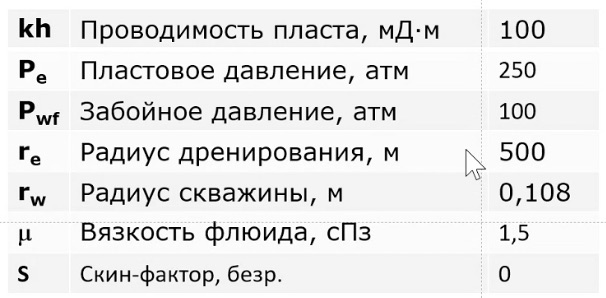
\includegraphics[width=0.4\textwidth]{input_for_Dupuy}

Здесь $P_e$ -- пластовое давление на границе области дренирования.

\beq
Q=\frac{kh}{18.41\cdot\mu}\frac{P_e-P_w}{\ln{\left(\dfrac{r_e}{r_w}\right)}+S}=
\frac{100\text{ мД}\cdot\text{м}}{18.41\cdot 1.5\text{ сПз}}\frac{250\text{ атм}-100\text{ атм}}{\ln{\left(\dfrac{500\text{ м}}{0.108\text{ м}}\right)}+0}\approx64\frac{\text{м}^3}{\text{сут}}
\eeq

\subsection{Задача 1}

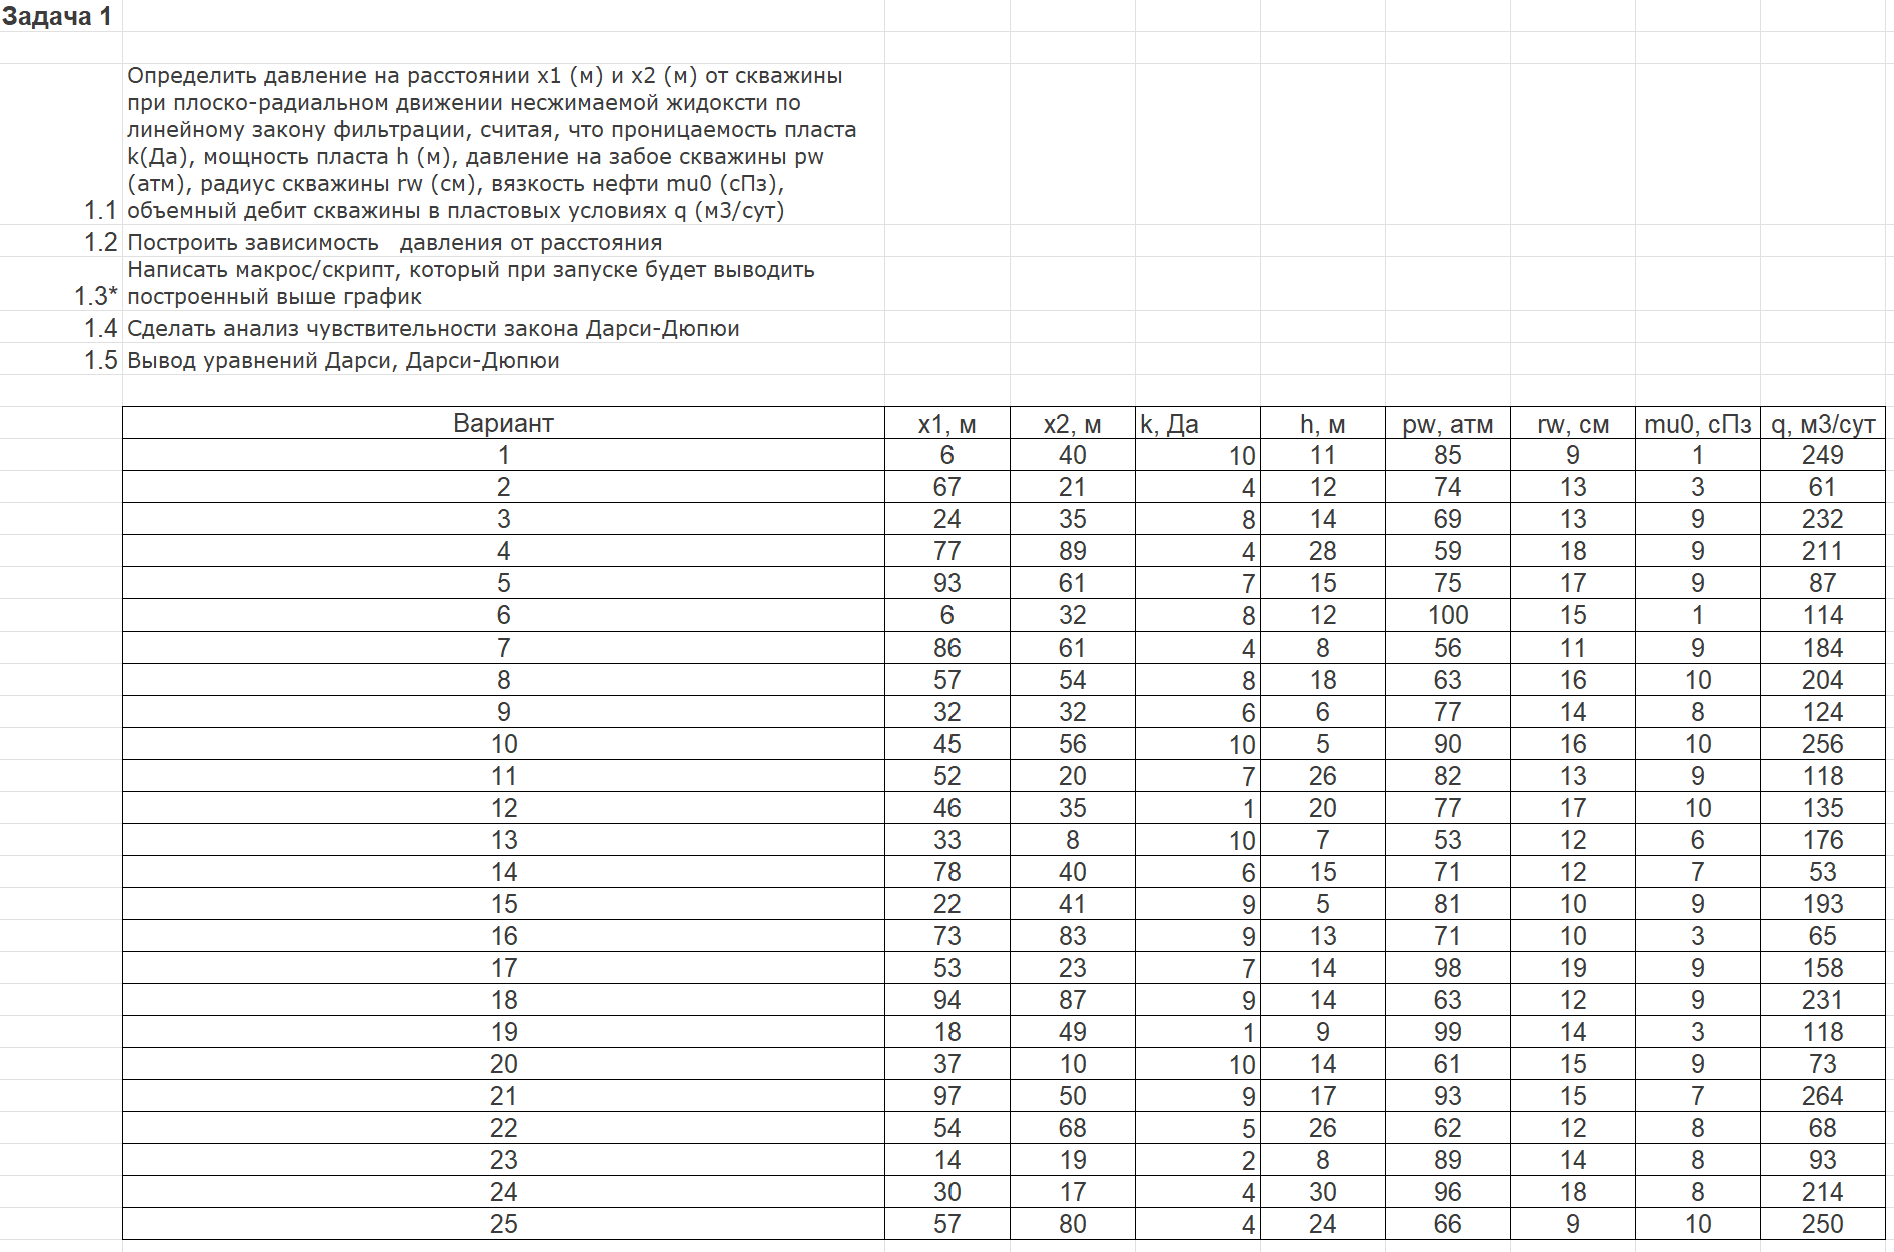
\includegraphics[width=\textwidth]{task1}

Вариант 16.

Давление на расстоянии $x_1$:
\begin{multline}
P_{x_1}=P_w+\frac{18.41\cdot Q\mu}{kh}\left(\ln{\left(\frac{x_1}{r_w}\right)+S}\right)
=\\=71\text{ атм}+\frac{18.41\cdot 65\dfrac{\text{м}^3}{\text{сут}}\cdot3\text{ сПз}}{9000\text{ мД}\cdot 13\text{ м}}\left(\ln{\left(\frac{73\text{ м}}{0.1\text{ м}}\right)}+0\right)\approx 71.2023\text{ атм}
\end{multline}

Давление на расстоянии $x_2$:
\begin{multline}
P_{x_1}=P_w+\frac{18.41\cdot Q\mu}{kh}\left(\ln{\left(\frac{x_2}{r_w}\right)+S}\right)
=\\=71\text{ атм}+\frac{18.41\cdot 65\dfrac{\text{м}^3}{\text{сут}}\cdot3\text{ сПз}}{9000\text{ мД}\cdot 13\text{ м}}\left(\ln{\left(\frac{83\text{ м}}{0.1\text{ м}}\right)}+0\right)\approx 71.2062\text{ атм}
\end{multline}

График зависимости давления от расстояния построен по ссылке: \href{https://colab.research.google.com/github/mualal/notebooks-source/blob/master/6_pressure.ipynb}{Open in Colab}.

\subsection{Что такое гидродинамическое моделирование?}

См. вводную лекцию.

\subsection{Уравнение пьезопроводности (без упругости пласта)}

См. вводную лекцию.

\subsection{Решение линейного стока/источника в однородном бесконечном коллекторе}

Для вывода решения используются безразмерные переменные. Например, безразмерные радиус, время и давление:

\beq
r_D=\frac{r}{r_w};\,\,\,\,\,\,\,\,t_D=\frac{kt}{\varphi c_t r_w^2};\,\,\,\,\,\,\,\,P_D=\frac{2\pi kh}{qB\mu}\left(p_i-p\right)
\eeq

Преимущества использования безразмерных переменных:

1) вид уравнений упрощается;

2) полученное один раз решение можно использовать для самых разных конфигураций;

3) безразмерные переменные -- основа для метода палеточной интерпретации.

Решение в безразмерных переменных, записанное через интегральную показательную функцию:
\beq
P_D(r_D,t_D)=-Ei\left(-\frac{r_D^2}{4t_D}\right),
\eeq
где
\beq
-Ei(-x)=\int\limits_{x}^{\infty}\frac{e^{-u}}{u}du.
\eeq

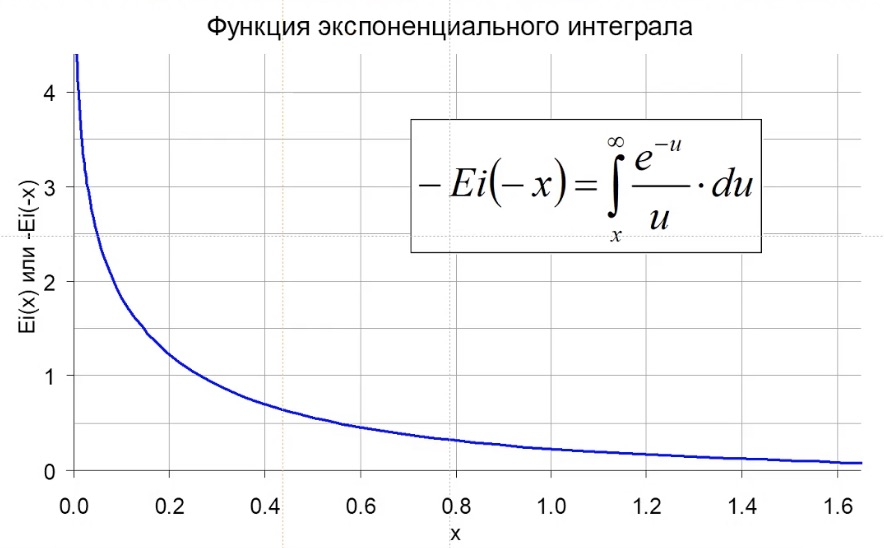
\includegraphics[width=0.5\textwidth]{exp_integral}

Логарифмическая аппроксимация решения при условии $\dfrac{r_D^2}{4t_D}\leqslant0.01$:
\beq
P_D(r_D,t_D)\approx -\frac{1}{2}\left[\ln\frac{\gamma r_D^2}{4t_D}\right]=\frac{1}{2}\left[\ln\frac{t_D}{r_D^2}+0.80907\right].
\eeq

Решение линейного стока:
\beq
P(r,t)=p_i-\frac{qB\mu}{2\pi kh}\left[-\frac{1}{2}Ei\left(-\frac{\varphi\mu c_t r^2}{4kt}\right)\right].
\eeq

Логарифмическая аппроксимация решения при условии $\dfrac{kt}{\varphi \mu c_t r^2}\geqslant25$:
\beq
P(r,t)\approx p_i-\frac{1}{2}\frac{qB\mu}{2\pi kh}\left[\ln\frac{kt}{\varphi\mu c_t r^2}+0.80907\right].
\eeq

\subsection{Что такое модель, или зачем нужно решать уравнение пьезопроводности?}

\beq
P(r,t)\approx p_i-\frac{1}{2}\frac{qB\mu}{2\pi kh}\left[\ln\frac{kt}{\varphi\mu c_t r^2}+0.80907\right].
\eeq

Уравнение пьезопроводности -- основа аналитических моделей пласта, использующихся в различных симуляторах (например, в Saphir).

\subsection{Задача 2}

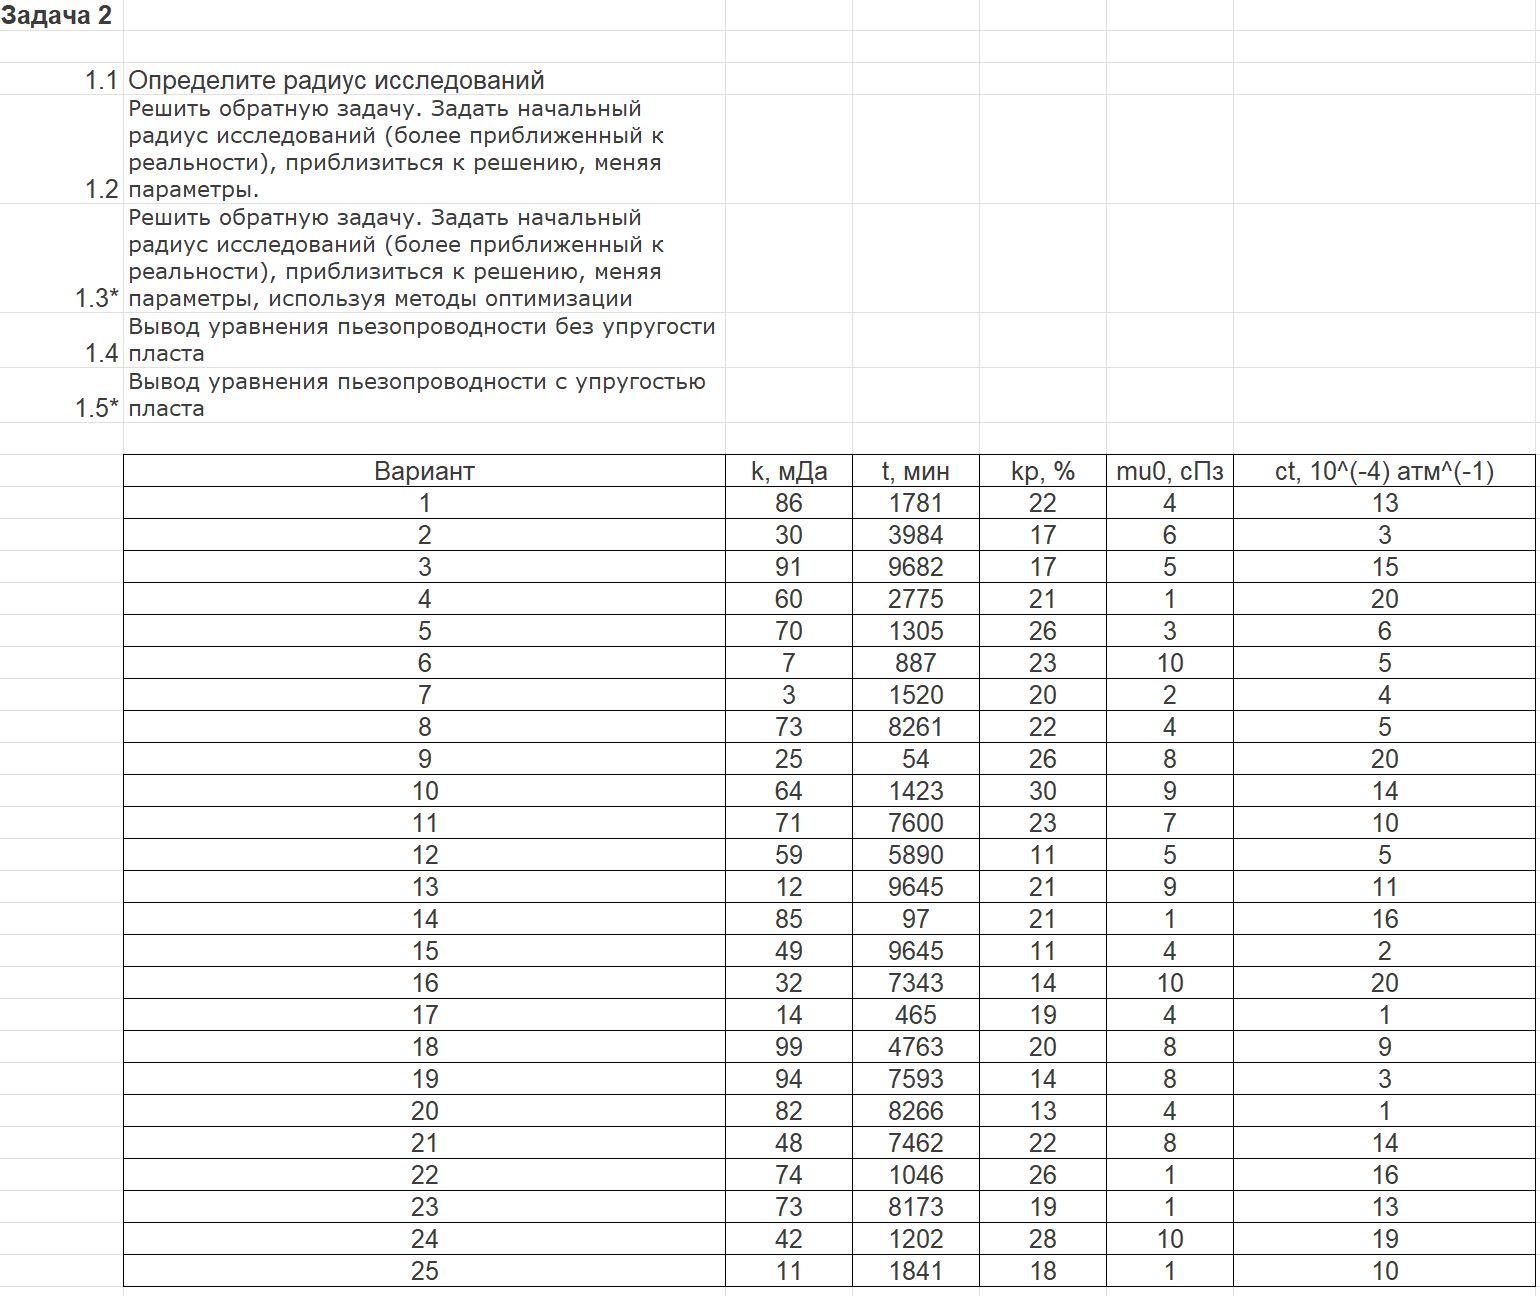
\includegraphics[width=\textwidth]{task2}
\textbf{Радиус исследований}

\beq
r_{inv}=0.037\sqrt{\frac{kt}{\varphi \mu c_t}}=0.037\sqrt{\frac{32\text{ мДа}\cdot 7343\text{ мин}}{0.14\cdot 10\text{ сПз}\cdot 20\cdot 10^{-4}\dfrac{\text{1}}{\text{атм}}}}\approx 338.95\text{ м}
\eeq
График зависимости радиуса исследования от произведения проницаемости и времени построен по ссылке: \href{https://colab.research.google.com/github/mualal/notebooks-source/blob/master/7_exploration_radius.ipynb}{OPEN IN COLAB}.
\\

\textbf{Решение обратной задачи}

Зададим радиус исследования $r_{inv}=100\text{ м}$, тогда:
\beq
kt=\varphi\mu c_t\left(\dfrac{r_{inv}}{0.037}\right)^2=0.14\cdot 10\text{ сПз}\cdot 20\cdot 10^{-4}\frac{1}{\text{атм}}\cdot \left(\frac{100\text{ м}}{0.037}\right)^{\!2}\approx 20452.89\text{ мДа}\cdot\text{мин}
\eeq
При проницаемости $k=32\text{ мДа}$, время исследования будет составлять:
\beq
t\approx\frac{20452.89\text{ мДа}\cdot\text{мин}}{32\text{ мДа}}\approx 639 \text{ мин}\approx10.65\text{ ч}.
\eeq


\subsection{Вывод уравнения пьезопроводности без упругости пласта (от Шеля Е.В.)}

Запишем ЗСМ для флюида:
\beq
\frac{\partial r_f}{\partial t}+\partial_i\left(r_f v_i^f\right)=0
\eeq

Закон Дарси в "<школьной"> форме:
\beq
Q=-\frac{\Delta p}{L}\frac{k}{\mu}S
\eeq

Закон Дарси в дифференциальной форме:
\beq\label{DarcyDiffShel}
W_i=-\frac{k_{ij}}{\mu}\partial_j p,
\eeq
где $W_i=\varphi v_i^f$ -- потоковая относительная скорость флюида.

Учитывая связь эффективной и истинной плотностей ($r_f=\varphi\rho_f$), перепишем ЗСМ для флюида:
\beq\label{ContinuityShel}
\frac{\partial\left(\rho_f\varphi\right)}{\partial t}+\partial_i\left(\rho_f\varphi v_i^f\right)=0
\eeq

Подставляя \eqref{DarcyDiffShel} в \eqref{ContinuityShel}, получаем:
\beq\label{GeneralPiezo}
\frac{\partial\left(\rho_f\varphi\right)}{\partial t}-\partial_i\left(\rho_f\frac{k_{ij}}{\mu}\partial_j p\right)=0
\eeq

--------------------------------------------------------------------

Замыкающее соотношение (связь плотности флюида и давления):
\beq\label{Zam1}
\rho_f=\rho_f^0\left(1+c_f\left(p-p_0\right)\right),
\eeq
где $c_f$ -- сжимаемость флюида (1/Па).


Замыкающее соотношение (связь пористости и давления):
\beq\label{Zam2}
\varphi=\varphi^0+c_{\text{п}}\left(p-p_0\right),
\eeq
где $c_{\text{п}}$ -- сжимаемость пор (не равно сжимаемости породы).

--------------------------------------------------------------------

Продифференцируем по времени замыкающее соотношение \eqref{Zam1}:
\beq\label{DiffZam1}
\frac{\partial\rho_f}{\partial t}=c_f\rho_f^0\frac{\partial p}{\partial t}
\eeq

Продифференцируем по пространству замыкающее соотношение \eqref{Zam1}:
\beq\label{GradZam1}
\partial_i\rho_f=c_f\rho_f^0\partial_i p
\eeq

Продифференцируем по времени замыкающее соотношение \eqref{Zam2}:
\beq\label{DiffZam2}
\frac{\partial\varphi}{\partial t}=c_\text{п}\frac{\partial p}{\partial t}
\eeq

Продифференцируем по пространству замыкающее соотношение \eqref{Zam2}:
\beq\label{GradZam2}
\partial_i\varphi=c_\text{п}\partial_i p
\eeq

--------------------------------------------------------------------

Раскрывая производные произведений в \eqref{GeneralPiezo}, получаем:
\beq\label{OpenGeneralContinuity}
\frac{\partial\rho_f}{\partial t}\varphi+\rho_f\frac{\partial\varphi}{\partial t}-\frac{k_{ij}}{\mu}\partial_j p\,\partial_i\rho_f-\rho_f\partial_j p\,\partial_i\!\left(\frac{k_{ij}}{\mu}\right)-\rho_f\frac{k_{ij}}{\mu}\left(\partial_i\partial_j p\right)=0
\eeq

Подставляя \eqref{DiffZam1}, \eqref{GradZam1}, \eqref{DiffZam2} и \eqref{GradZam2} в \eqref{OpenGeneralContinuity}, получаем:
\begin{multline}\label{Expanded}
c_f\rho_f^0\frac{\partial p}{\partial t}\varphi+\rho_f c_\text{п}\frac{\partial p}{\partial t}-\frac{k_{ij}}{\mu}\partial_j p\,c_f\rho_f^0\,\partial_i p-\frac{\rho_f}{\mu}\partial_j p\,\partial_i k_{ij}+\\+\rho_f\,\partial_j p\,k_{ij}\frac{\partial\mu}{\partial p}\frac{1}{\mu^2}\partial_i p-\rho_f\frac{k_{ij}}{\mu}\left(\partial_i\partial_j p\right)=0
\end{multline}

--------------------------------------------------------------------

Перед анализом физических уравнений всегда делают масштабный анализ, чтобы понять, какие слагаемые в уравнении важны, а какие не важны (пример: уравнение Навье-Стокса с числами Струхаля, Эйлера, Рейнольдса, Фруда).

Спойлер: ГДМ симуляторы не решают уравнение пьезопроводности в классическом виде, а решают закон сохранения массы, в который они подставляют закон Дарси.

Далее необходимо выделить характерные масштабные факторы, обезразмерив каждую из функций в уравнении.

Введём безразмерное давление $\tilde{p}$ такое, что:
\beq
p=\tilde{p}\cdot p_0,
\eeq
где $p_0$ -- пластовое давление.

Введём безразмерное расстояние $\tilde{r}$ такое, что:
\beq
\vec{r}=\tilde{r}\cdot L,
\eeq
где $L$ -- некое характерное расстояние (например, между скважинами).

Введём безразмерную проницаемость $\tilde{k}_{ij}$ такую, что:
\beq
k_{ij}=\tilde{k}_{ij}\cdot k_0,
\eeq
где $k_0$ -- некая характерная проницаемость.

Введём безразмерную вязкость $\tilde{\mu}$ такую, что:
\beq
\mu=\tilde{\mu}\cdot\mu_0,
\eeq
где $\mu_0$ -- некая характерная вязкость.

Все безразмерные функции (с волной) порядка единицы.

--------------------------------------------------------------------

Перепишем \eqref{Expanded} в введённых безразмерных величинах, разделив обе части этого уравнения на $\rho_f^0$:
\begin{multline}
\frac{\partial p}{\partial t}\left(\varphi c_f+\frac{\rho_f}{\rho_f^0}\cdot c_\text{п}\right)-\frac{k_0}{\mu_0}\frac{p_0^2}{L^2}c_f\frac{\tilde{k}_{ij}}{\tilde{\mu}}\,\tilde{\partial}_i\tilde{p}\,\tilde{\partial}_j\tilde{p}-\frac{\rho_f}{\rho_f^0}\frac{k_0\,p_0}{\mu_0L^2}\frac{\tilde{k}_{ij}}{\tilde{\mu}}\,\tilde{\partial}_j\tilde{p}\,\tilde{\partial}_i\tilde{k}_{ij}+\\+\frac{\rho_f}{\rho_f^0}\frac{p_0\,k_0}{L^2\mu_0}\,\tilde{\partial}_j\tilde{p}\,\tilde{k}_{ij}\frac{\partial\tilde{\mu}}{\partial\tilde{p}}\frac{1}{\tilde{\mu}^2}\,\tilde{\partial}_i\tilde{p}-\frac{\rho_f}{\rho_f^0}\frac{k_0}{\mu_0}\frac{p_0}{L^2}\,\frac{\tilde{k}_{ij}}{\tilde{\mu}}\left(\tilde{\partial}_i\tilde{\partial}_j\tilde{p}\right)=0
\end{multline}

Вынесли все масштабные множители. Далее делим обе части уравнения на множитель перед старшей производной $\left(\text{на }\frac{k_0\,p_0}{\mu_0\,L^2}\right)$, т.е. обезразмериваем уравнение:
\begin{multline}\label{PiezoEqDiv}
\frac{\mu_0L^2}{k_0p_0}\cdot\frac{\partial p}{\partial t}\left(\varphi c_f+\frac{\rho_f}{\rho_f^0}\cdot c_\text{п}\right)-p_0c_f\frac{\tilde{k}_{ij}}{\tilde{\mu}}\,\tilde{\partial}_i\tilde{p}\,\tilde{\partial}_j\tilde{p}-\frac{\rho_f}{\rho_f^0}\frac{\tilde{k}_{ij}}{\tilde{\mu}}\,\tilde{\partial}_j\tilde{p}\,\tilde{\partial}_i\tilde{k}_{ij}+\\+\frac{\rho_f}{\rho_f^0}\frac{\partial\tilde{\mu}}{\partial\tilde{p}}\frac{1}{\tilde{\mu}^2}\tilde{k}_{ij}\,\tilde{\partial}_j\tilde{p}\,\tilde{\partial}_i\tilde{p}-\frac{\rho_f}{\rho_f^0}\frac{\tilde{k}_{ij}}{\tilde{\mu}}\left(\tilde{\partial}_i\tilde{\partial}_j\tilde{p}\right)=0
\end{multline}

--------------------------------------------------------------------

Сделаем 3 важных приближения:
\begin{enumerate}
	\item $p_0 c_f\ll 1$ (прикинем: сжимаемость воды порядка $10^{-5}\text{ атм}^{-1}=10^{-10}\text{ Па}^{-1}$; характерные значения давлений на глубинах, равных нескольким километрам, составляют сотни атмосфер; таким образом, произведение порядка $10^{-3}$, что много меньше единицы; но такое приближение не работает для газа: для него рассматриваемое произведение порядка единицы); это приближение фактически равносильно приближению $\rho_f\approx\rho_f^0$;
	\item $\tilde{\partial}_i\tilde{k}_{ij}\ll 1$ (считаем, что на характерном масштабе задачи по данному направлению проницаемость изменяется незначительно, не больше 10 процентов);
	\item $\dfrac{\partial\tilde{\mu}}{\partial\tilde{p}}\ll 1$ (считаем, что отмасштабированный график проницаемости от давления пологий -- этот факт подтверждается экспериментально -- вязкость слабо зависит от давления)
\end{enumerate}

Тогда уравнение \eqref{PiezoEqDiv} перепишется в следующем виде (убрали слагаемые с пренебрежимо малыми множителями в рамках сделанных приближений и вернулись от безразмерных функций с волной к обычным функциям):
\beq
\frac{\partial p}{\partial t}\underbrace{\left(\varphi c_f+c_\text{п}\right)}_{c_t}-\frac{k_{ij}}{\mu}\partial_i\partial_j p=0
\eeq
(заметим, что если есть анизотропия проницаемости, то лапласиана в уравнении не будет).

Получаем классическое уравнение пьезопроводности:
\beq
\frac{\partial p}{\partial t}-\frac{k_{ij}}{\mu c_t}\partial_i\partial_j p=0,
\eeq
где $c_t$ -- это полная сжимаемость.

Замечание. Но есть литература, в которой $c_t=c_f+\frac{c_\text{п}}{\varphi}$, тогда уравнение пьезопроводности будет выглядеть так:
\beq
\frac{\partial p}{\partial t}-\frac{k_{ij}}{\mu\varphi c_t}\partial_i\partial_j p=0
\eeq

--------------------------------------------------------------------

Пусть тензор проницаемости изотропен $k_{ij}=k_0\cdot\delta_{ij}$, тогда:
\beq
\frac{\partial p}{\partial t}-\frac{k_0}{\mu c_t}\delta_{ij}\,\partial_i\partial_j p=0\Leftrightarrow\frac{\partial p}{\partial t}-\frac{k_0}{\mu c_t}\Delta p=0
\eeq
(получили всем известный вид уравнения пьезопроводности).

\end{document}
